\part{User Guide}
\chapter{Administrative Site Usage}

After you have completed the \hyperref[software_setup]{\textcolor{blue}{\underline{Software Setup}}}, you are ready to begin using the site. This will entail creating creating the initial admin user.

\section{Creating the Initial Admin User}

To create the inital admin user, simply visit /setup/ to be prompted for your administrator information. For example, if your website is https://portales\_theatre.com, browse to https://portales\_theatre.com/setup/.

Once you enter the administrative information for the the admin user and click on Create Admin, your initial admin account will be created and is ready to log in with. To test this, simply click on ``Login'' at the top right and log in with your admin user's email and password.

\section{Administrative Area}

After creating the admin user and logging in, you will be able to enter the administrative area of the site by clicking on the ``Admin Area'' as shown in figure \ref{fig:admin_area_link}.

\begin{figure}[ht]
    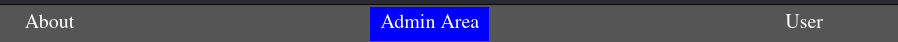
\includegraphics[width=16cm]{images/chapter2/admin area link}
    \caption{Admin Area Selection}
    \label{fig:admin_area_link}
\end{figure}

Once selected, the site administration home will load. The site administration area provides you with selections to manage the site. Currently this only includes managing users and plays, but more options could be added in later. For ease of navigation, the buttons in the middle of the screen and the links on the left side of the screen both lead to the same sections of the site. A picture of the admin area can be seen in figure \ref{fig:admin_area_home}.

Clicking on ``Users'' will allow you to manage the users of the site as described in \hyperref[sec:managing_users]{\textcolor{blue}{\underline{Managing Users}}}.

Clicking on ``Plays'' or ``Schedule'' will allow you to create and manage plays for the site as described in \hyperref[sec:managing_plays]{\textcolor{blue}{\underline{Managing Plays}}}.

Clicking on ``Leave Admin'' or ``Back'' will return you to the main page of the site.

Clicking on ``Logout'' will log you out of your administrative account and return you to the main page of the site.

Clicking on ``Admin Home'' will return you to the main page of the admin home.

\begin{figure}[ht]
    \centering
    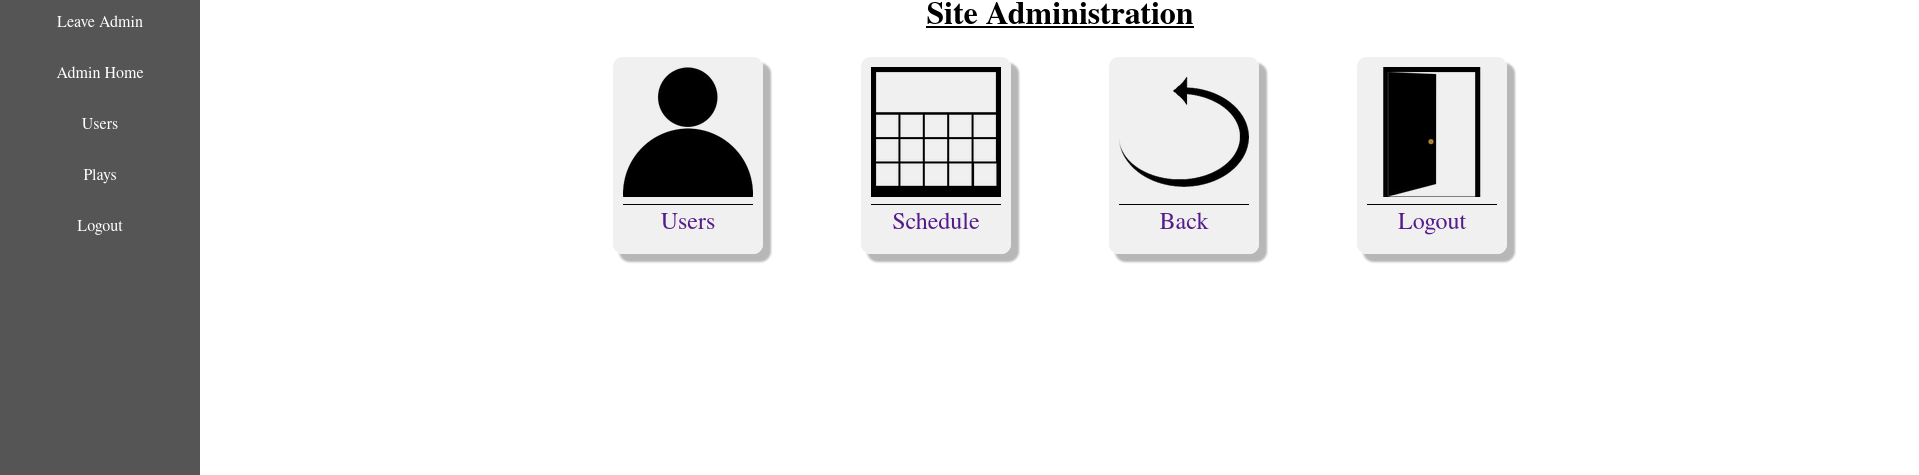
\includegraphics[width=12cm]{images/chapter2/admin area home}
    \caption{Admin Area Home Screen}
    \label{fig:admin_area_home}
\end{figure}

\section{Managing Users}\label{sec:managing_users}

When you select the ``Users'' link or card, you will be presented with the users screen. See figure \ref{fig:admin_area_user_home} for an example of what this page looks like. This screen allows you to view all current users of the site. When you first open this screen, you should only see a few users (likely just yourself). To make it easy to determine at a glance who has administrative permissions and who does not, the users are clearly divided into Administrators and Users. As users register for the site, or as you create other users on the site, they will appear here.

\begin{figure}
    \centering
    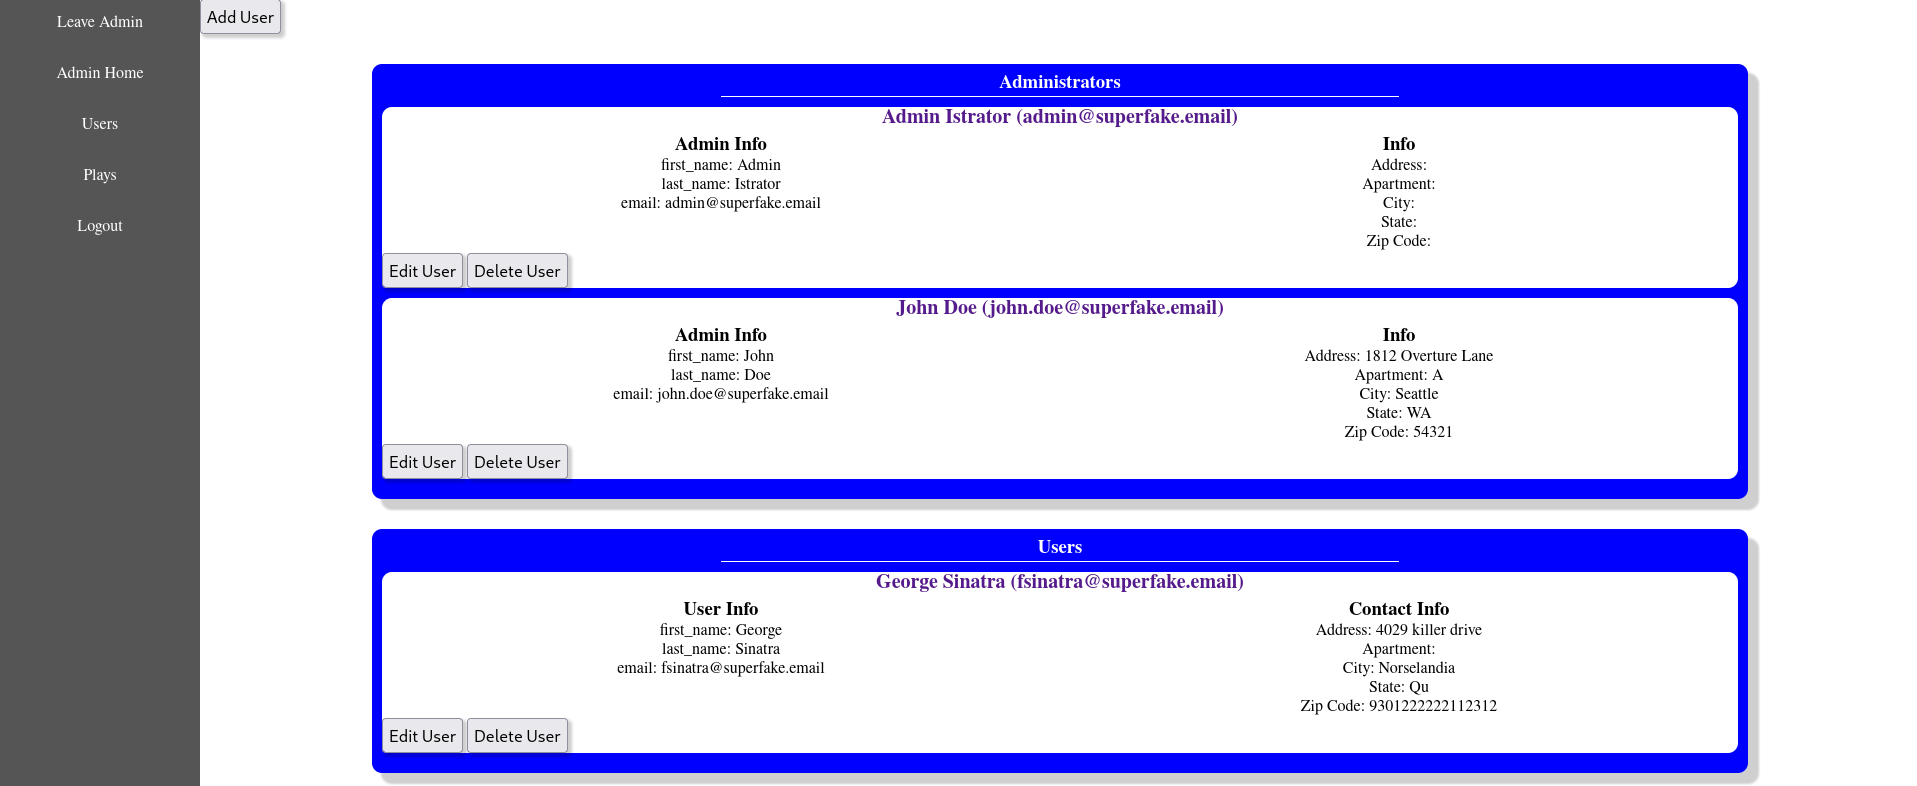
\includegraphics[width=12cm]{images/chapter2/admin area users home}
    \caption{Users Administration Home}
    \label{fig:admin_area_user_home}
\end{figure}

Clicking on the ``Add User'' button will walk you through the new user setup. This entails providing the email, first name, last name, address information, and password for the user. You may optionally set the user to be an administrator during user creation.

Each user on the page has an ``Edit User'' and ``Delete User'' button associated with them. Clicking on ``Edit User'' will display the user information and allow you to make changes to the user's information. Clicking on ``Delete User'' will delete the user from the system. Do note that deleting the user will not remove any reservations that they have made.

\section{Managing Plays}\label{sec:managing_plays}

Selecting ``Plays'' or ``Schedule'' will bring you to the play modification area. This section of the site allows you to create, modify, and manage plays. This page can be seen in figure \ref{fig:admin_area_play_home}.

\begin{figure}[ht]
    \centering
    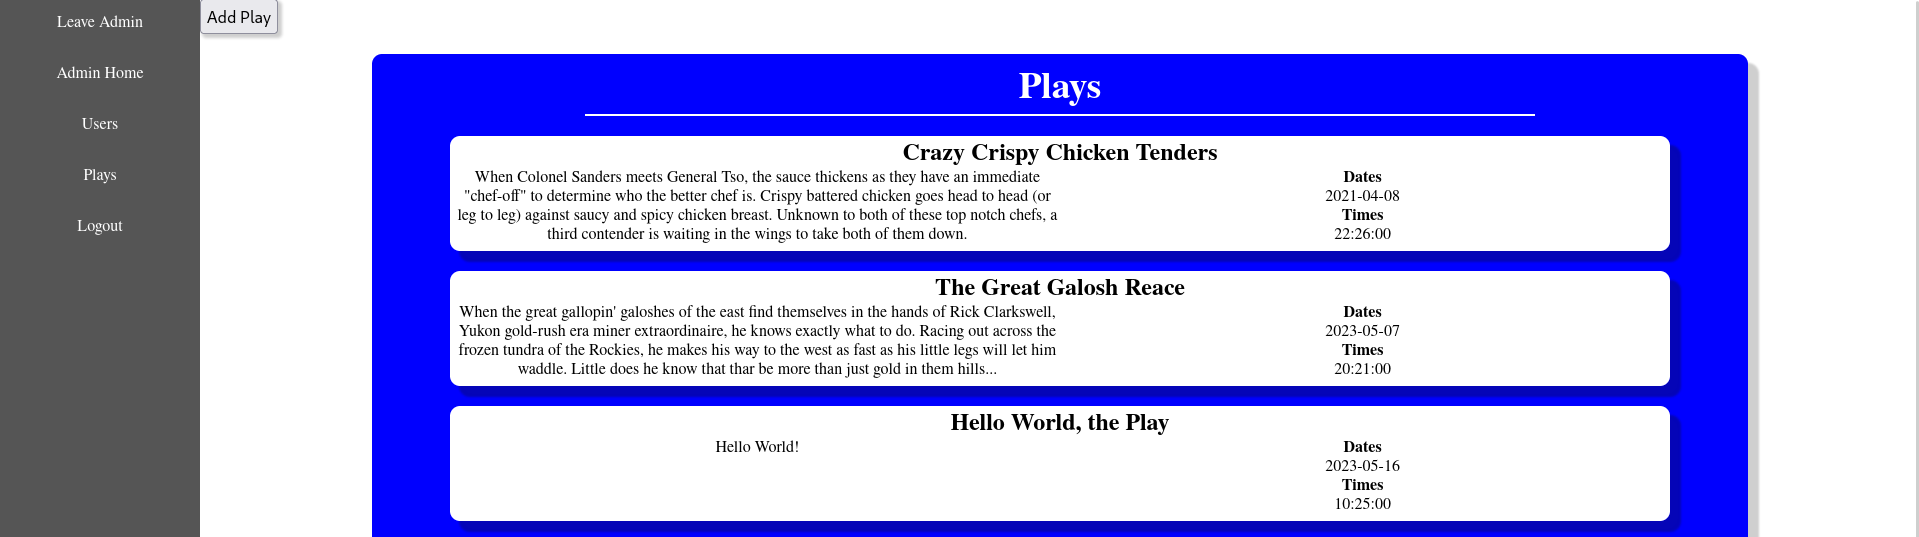
\includegraphics[width=14cm]{images/chapter2/admin area play home}
    \caption{Play Administration Home}
    \label{fig:admin_area_play_home}
\end{figure}

When first opening this page, there will be no plays present to modify. Clicking on the ``Add Play'' button in the top left will walk you through the play creation. Creating a play requires a date, a time, a name, and a description. This play creation form can be seen in figure \ref{fig:admin_area_create_play}

\begin{figure}[ht]
    \centering
    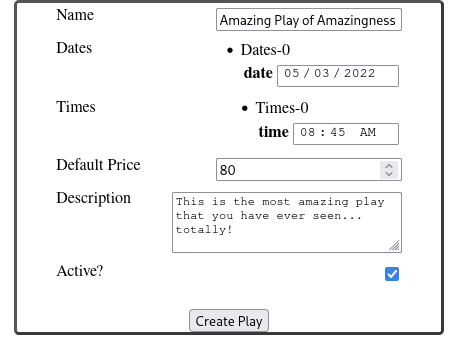
\includegraphics[width=6cm]{images/chapter2/admin area create play form}
    \caption{Creating a Play}
    \label{fig:admin_area_create_play}
\end{figure}

Once a play has been created, you can click on it from the play administration page to view information about the play and make modifications to the play. View figure \ref{fig:admin_area_modify_seating} and figure \ref{fig:admin_area_modify_details} for an example of what this page looks like. From the play modification screen, you will be able to view and modify the following information about the play.

\begin{enumerate}
    \item Play Name
    \item Play Time
    \item Play Date
    \item Default Seat Price
    \item Play Description
    \item Whether or not the play is active
    \item Individual Seat Pricing
\end{enumerate}

\begin{figure}[ht]
    \centering
    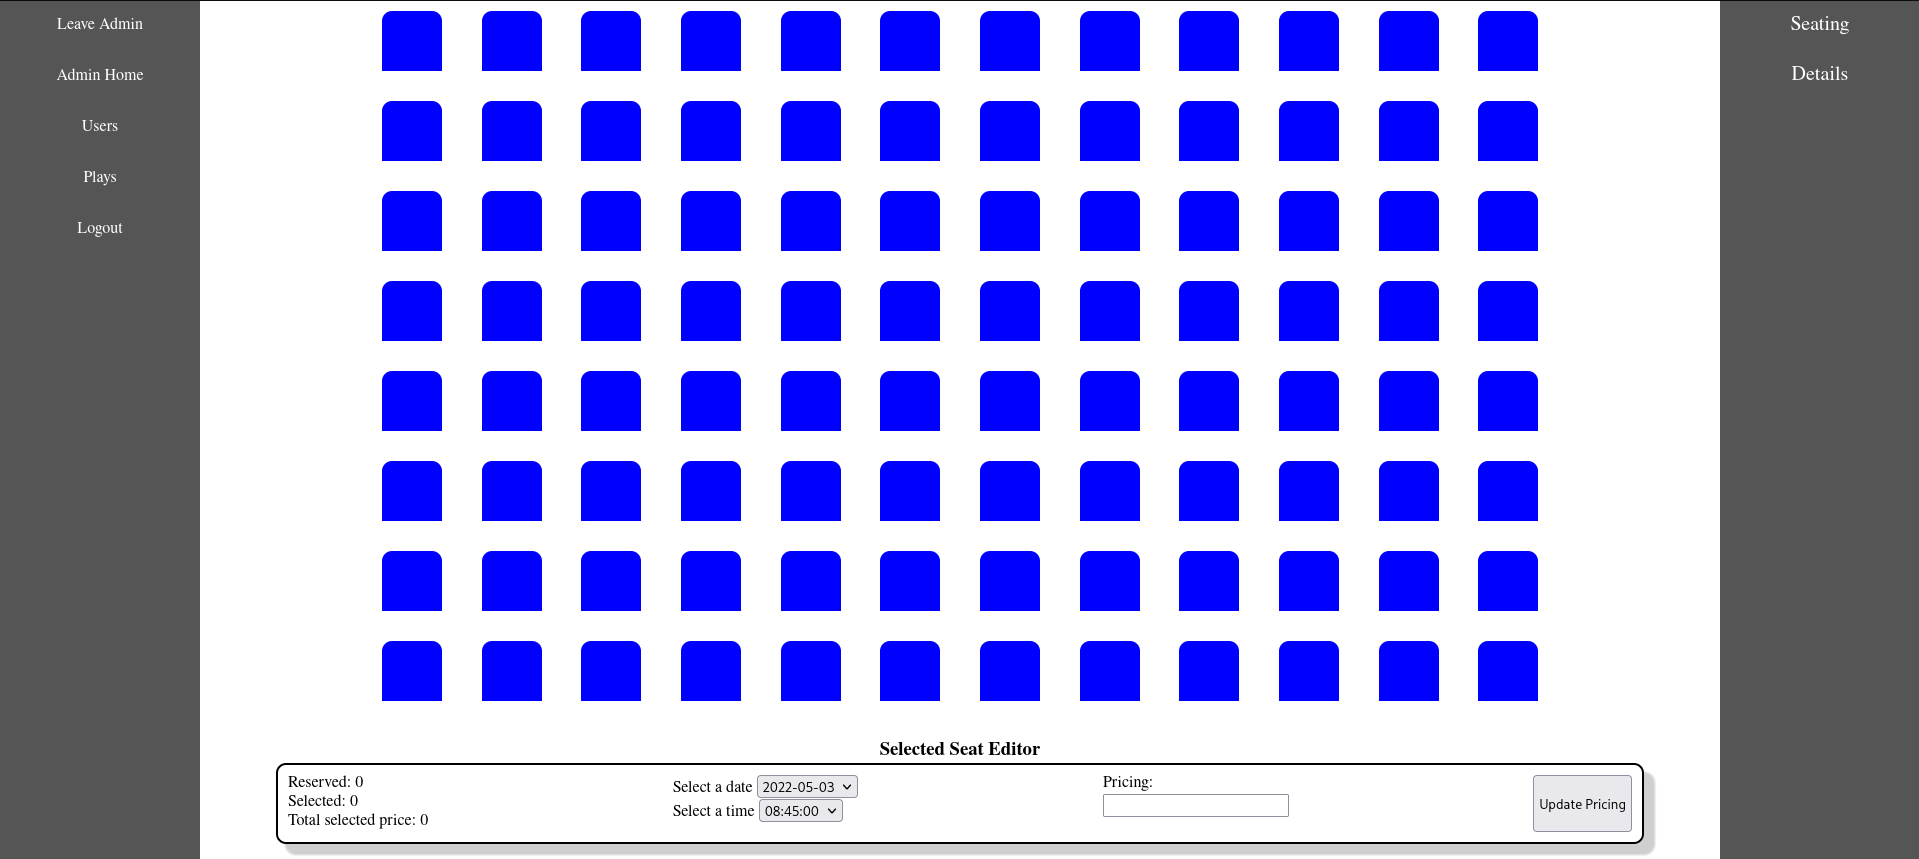
\includegraphics[width=14cm]{images/chapter2/admin area modify seating}
    \caption{Play Seating Modification}
    \label{fig:admin_area_modify_seating}
\end{figure}

\begin{figure}[ht]
    \centering
    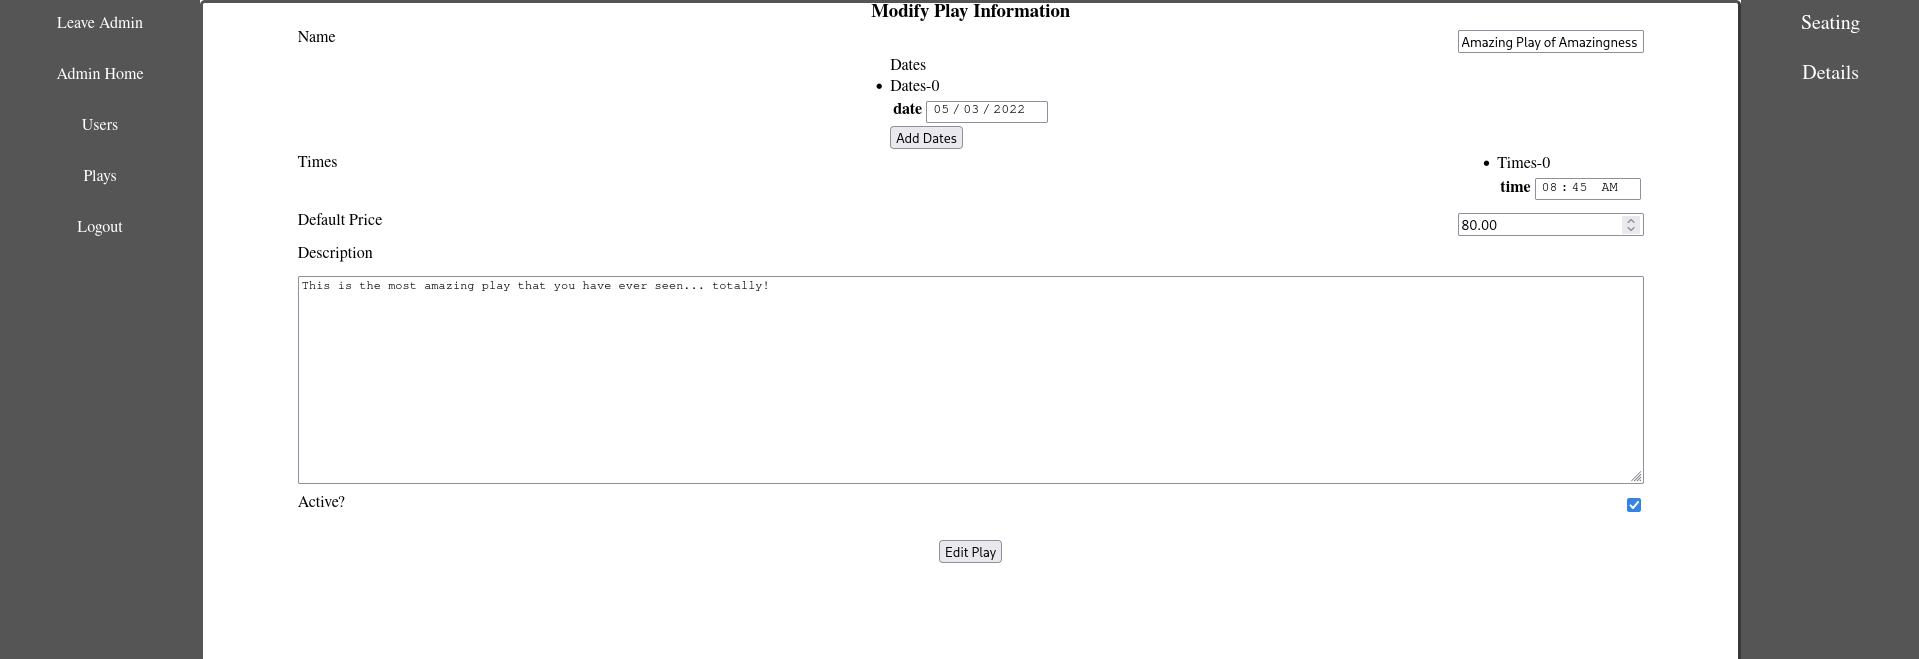
\includegraphics[width=14cm]{images/chapter2/admin area modify details}
    \caption{Play Detail Modification}
    \label{fig:admin_area_modify_details}
\end{figure}

Individual seat pricing is modified on the first screen shown when selecting a play. To modify an individual seat's pricing (or a group of seats), click on the seats you wish to modify. They will turn green indicating that they have been selected as seen in figure \ref{fig:admin_area_seat_selected}.

\begin{figure}[ht]
    \centering
    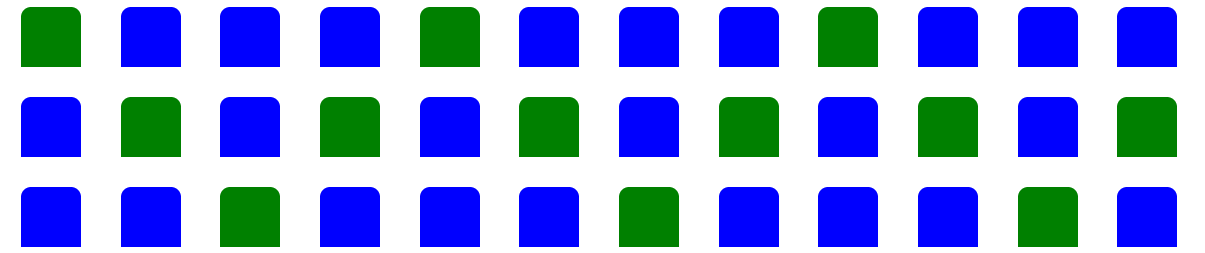
\includegraphics[width=12cm]{images/chapter2/admin area seat selected}
    \caption{Play Seating Selection.}
    \label{fig:admin_area_seat_selected}
\end{figure}

Once the seats have been selected, you can enter the seating price in the selected seat editor at the bottom of the screen and change the pricing of all the selected seats. If you wish to modify the pricing of all the seats at the same time, simply click on the details tab and change the default price. Once you have completed your modifications to the play, you can leave the administration area and view the play as a customer would view it (assuming you have left the play active).

\begin{figure}[ht]
    \centering
    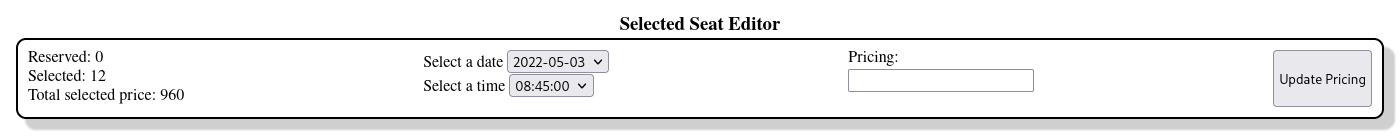
\includegraphics[width=12cm]{images/chapter2/admin area seat editor}
    \caption{Play Seating Editor}
    \label{fig:admin_area_seat_editor}
\end{figure}
